\documentclass[a4paper,12pt]{article}

%% Language and font encodings
\usepackage[english]{babel}
\usepackage[utf8x]{inputenc}
\usepackage[T1]{fontenc}

%% Sets page size and margins
\usepackage[a4paper,top=3cm,bottom=2cm,left=3cm,right=3cm,marginparwidth=1.75cm]{geometry}

%% Useful packages
\usepackage{amsmath}
\usepackage{graphicx}
\usepackage[colorinlistoftodos]{todonotes}
\usepackage[colorlinks=true, allcolors=blue]{hyperref}
\begin{document}
\begin{titlepage}
\begin{center}
		{\Large \textbf{Ludwig-Maximilians-Universität München}} \\
	\vspace{35mm}
{\bfseries\LARGE{Factor Immobility and Regional Impacts of Trade Liberalization: Evidence on Poverty from India}} \\{\bfseries\large{by Petia Topalova}} 
			\vspace{10mm}\\
            {\Large Advanced Seminar in Empirical International Trade } \\
			\vspace{2mm}
            {\Large{Bakai Baiazbekov
		\renewcommand\thefootnote{*}\footnote{B.Baiazbekov@campus.lmu.de}}}\\
        {\today}	\\
		\vspace{8mm}
		\begin{figure}[h] 
        \begin{center}

\includegraphics[width=0.6\textwidth]{lmu_siegel.png} \
\end{center}
\end{figure}%
	\end{center}

\end{titlepage}


\pagenumbering{Roman}
\setcounter{page}{2}
\tableofcontents  
\newpage



\pagenumbering{arabic}
\setcounter{page}{1}

\section{Introduction}
Self-control problems change the logic of agency theory by partly aligning the interests of a firm and a worker. Now, both the firm and worker value contracts which extract future effort. 

Agency theory emphasizes a tension between workers and firms. Because employers provide insurance, workers do not benefit fully from their effort. Such situation creates a moral hazard that workers do not work as hard as the employer wants them to \cite{Holm79}. This analysis suggests that there is another tension at work -  self-control. Self-control problems means that workers often do not work as hard as they themselves would like to. However, when looking to the future , they would like to work hard, and when the future arrives, they may end up slacking. 

This seminar paper focuses on the test of self-control problems to see the correlation between incentives and commitment to savings. 

Self-Control at work differs from the self-control in other aspects such as savings, alcohol consumption or smoking. In many of these contexts, the market provides commitment to the consumer demands to create a new institution. However, worker self-control problems directly hurt employer profits. The same features that reduce the moral hazard incentive contracts and job design features such as fixed hours of work -  can also reduce the self-control problems. In other words, the employer has both the means and motives to implicitly provide commitment devices. 

The  seminar  paper consists of two papers and it is  structured  as  follows: section 2 Introduces the summary, experimental design, results and critical assessment. Section 3 describes with summary of second paper, self-control in alcohol consumption, and continues experimental design and reflects my  own critical thoughts on the model.  


\section{Paper1 "Self-Control at Work"}


\subsection{Summary}

The discussion of this paper composes such questions: Do job features such as:  assembly lines, production minimums, rigid work hours and large amount of punishments for even small failures in behavior have self control benefits? Why the movement from farm to factory work has typically been accompanied by increases in labor productivity? Are workplace incentive contracts , which often embody high -powered incentives in some form, at least partially structured to provide self-control benefits? Could organization of production itself serve to mitigate self- control problems? 

It is important to see the correlation between employers, who provide the insurance, and workers, who don't fully benefit from their effort. In other words, workers do not work as hard as the employer would like them to. Therefore, to mitigate the moral hazard, incentive contracts and job design exist. 

In this paper, author used a model to distinguish the behavior of time-consistent and time-inconsistent workers. In this model, workers must be compensated for a sharpening of incentives: they face extra risk. Sophisticated workers who are aware of their self-control problem will value sharper incentives as a way to motivate future selves. Therefore, the authors made an experiment, where each day workers offered a choice between two types of incentive working methods. Firstly, the piece rate method and dominated contract that pays less than piece rate for low output but for high output it pays the same. In this situation, sophisticated workers may voluntarily choose a dominated contract. One day in a week, workers get the payment for their effort. In addition, the contract choice happens either before work or previous evening(after work). 

In order to predict the demand for dominated contracts, this model suggests that the timing of pay affects the effort. As a payday gets closer, the source of the self-control problem reduces rewards of work and cost of work. Moreover, workers with greater self control problems showed both larger payday effects and a greater desire for dominated contracts. 

The main goal of this experiment was, firstly, to test \textit{the demand of dominated contracts}, where on random days workers were offered the option to choose a target for the day. As a result, on average, workers selected positive targets, where in 36 percent of the time, they behaved to choosing dominated contracts.  This option to choose dominated contract increased production and earnings at 6 percent.

Second goal was to test \textit{the impact of paydays}, where workers were randomized into different payday groups. All were paid weekly but the exact day of payment varied. Results showed that worker output is 8 percent higher on paydays than at the beginning of the weekly pay cycle. The effect of this consequence corresponds to a 24 percent increase in the piece rate or about additional year of education. 

Third goal was to find heterogeneity in the extent of the payday and contract effects. Workers with above mean payday effects are 49 percent more likely to choose dominated contracts. This option gave increased output by 9 percent. It means that, for these workers, dominated contracts have production impacts comparable to an 85 percent increase in the piece rate wage. 

Further discussed, the reasons why workers are no more likely to select dominated contracts,where take-up on the morning and the evening of workday is similar. First, workers faced some output uncertainty, for instance, it can be from network speed fluctuations or uncertain commute times(arrival time to office). When such uncertainty is low, workers demand targets, with high probability, the evening before work than the morning. In addition, as workers gain experience, the correlation between payday effects and the choice of dominated contracts increases. For instance, after 2 months of experience, workers with high payday effects are 73 percent more likely to select dominated contracts than workers with low payday effects. These results indicate that workers will demand incentives that help them overcome self-control problems. The dominated contract helps to solve the self-control problem by creating high-powered incentives, like many sales firms provide discrete bonuses for meeting targets. Otherwise, if workers are risk-averse and dislike the high-powered incentives on output, self-control problems make firms more likely to install and implement costly technologies to measure effort. 

Overall, the experiment showed that many workers are present biased. It substantially affects their effort and that they are sophisticated enough to choose dominated contracts. Authors showed that present bias among workers will lead firms to offer higher-powered incentives and that sufficiently strong present-bias reverses the standard partial insurance result. The distribution of output dominates the distribution of wages and,therefore, present-biased workers exert more effort and produce more output as employees than as self-employed owner-operators. 




\subsection{Experimental Design}

\textbf{Experimental Context }: 
The main goal of the experiment was to assess the empirical relevance and magnitude of time inconsistency. 
For the experiment data was pooled from Indian data entry company, where workers used data entry software to type information from scanned images into fields on their computer. The software provided them with information on their own output with about 15-minute delay. Following standard practice in the data entry industry, workers were paid piece rates based on the number of accurate fields entered. The accuracy was measured using dual entry of data, with manual checks of discrepancy by separate quality control staff. Workers were paid a piece rate of Rs.0.03(rupees) for each accurate field entered and small fix rate daily for showing-up fee of Rs.15 that constituted about 8 percent of their compensation. They earned zero on days they were absent. 

The earnings were measured by the following equation $w(e) = Rs.15 + Rs.0.03e$. Workers were payed one time in three different days: Tuesday,Thursday and Saturday. This helped to control for other day-of-the-week factors that might affect effort, such as a post/pre-weekend effect.   

They were recruited and hired by standard process:  Via announcements resumes were submitted by walk- ins. Applicants were required to be at least 18th years old. From submitted applicants average age was 24 years old and mainly three-quarters were male. They completed in average 13 years of education and had already introduced on how to use computer and had email addresses prior to starting new job. Many of the hired workers were from surrounded villages and travel time to working place was up to 2 hours in one direction. New recruits received about 2 weeks of training before contract randomizations began and were paid flat rate. During the next 4 days, they worked under assignment to the control contract with wage schedule $w(e)$. Moreover, they were assigned to the dominated contract for 2 days under the low and medium targets. This opportunity is good to observe their production under both types of incentive schemes before beginning contract randomizations. 

\textbf{A Simple Model}


In this simple model was derived empirically testable predictions to distinguish the behavior of time-consistent and time-inconsistent workers. Assume that worker \textit{i} has the period utility function $y_t-\alpha^i c(e_t)$, where $y_t$ is income received in period \textit{t}, $e_t$ is effort in period \textit{t}, $c(.)$ is the cost of effort and $\alpha^i \succ 0$ reflects individual variation in effort costs. $D^i(t)$ denotes for worker \textit{i}'s discount factor, where $D^i(t)  \epsilon  {D^C(t),D^I(t)}$. Time-consistent workers discount the future using an exponential discount factor: $D^C(t)=\delta^t$. Time-inconsistent workers have a hyperbolic discount factor $D^I(t)$ and for any delay $D^I(t+s)/D^I(t)$. 

\textit{Optimal effort} : under quasi-linear utility, optimal effort in each period is separable from effort choice to other period. So, in period \textit{t-k} the worker's preferred period \textit{t} effort maximizes $$\max_{e}[D^i(T-t+k)w(e)-D^i(k)c(e)].$$
by first-order condition :$$c\prime(e^i_{t|t-k})=\frac{D^i(T-t+k)}{D^i(k)}b$$

where \textit{b} is the piece rate in the affine contract \textit{w(e)}. 


Proposition 1 (Pay cycle effect) The proportional increase in output from period $t$ to $t+1$ is given by 
\begin{equation}
 \frac{e_{t+1 \vert t+1}^i-e_{t \vert t}^i}{e_{t \vert t}^i}=\epsilon \left[ \frac{D^i (T-t-1)-D^i(T-1)}{D^i(T-t)}\right]
\end{equation}

where $\epsilon$ is the elasticity of output with respect to the piece rate. The term in brackets reduces to $(\frac{1}{\delta}-1)$ if workers are exponential discounters and is greater than $(\frac{1}{\delta}-1)$ if they are time-inconsistent. It implies that output increases over the pay cycle will be larger for time-inconsistent workers than for time-consistent ones. 
\begin{figure}[h]
\centering
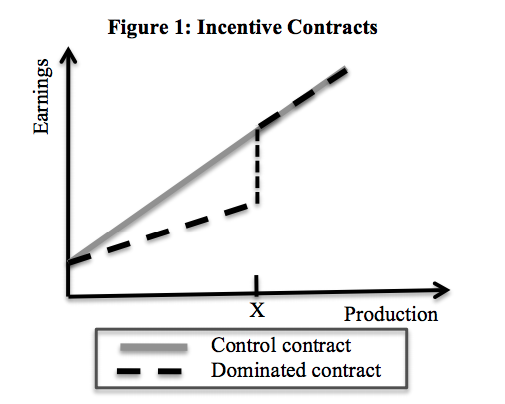
\includegraphics[width=0.7\textwidth]{Figure1_1.png}
\caption{\label{fig:Figure1}}
\end{figure}

Proposition 2 (Demand for dominated contracts, bounds on time inconsistent)
\textit{a.} Suppose that in period \textit{t-k} workers are offered the following dominated wage schedule, which allows them to choose a target output level $X_{t|t-k}$ for period \textit{t}: 
\begin{equation}
v_{t|t-k}(e)=\{(a+b^pe ; a+be  ) 
\end{equation}

where $0\leq b_p<b$. Time-inconsistent workers period \textit{t-k} selves will strictly prefer $v_{t|t-k}(.)$ over $w(.)$ and will choose $X_{t|t-k}\epsilon(e^i_{t|t}, e^i_{t|t-k})$. 

\textit{b.} Defined $x^i_{t|t-k}$ as the proportional increase in output under $v_{t|t-k}(.)$ relative to $w(.) at time \textit{t}$. Then $x^i_{t|t-k}$  is bounded above by elasticity times the level of time inconsistency between periods \textit{t-k} and \textit{t}: 

\begin{equation}
x^i_{t|t-k} \leq \epsilon [\frac{\frac{D^i(T-t+k)}{D^i(k)} {\frac{D^i(T-t)}{D^i(0)}}} - 1]
\end{equation}


Proposition 3 (Correlation of pay cycle and dominated contract effects). 
Assumed some workers are time-consistent exponential discounters with discount function $D^C(.)$ and others are time inconsistent with discount function $D^I(.)$. Then the magnitude of output increase over the pay cycle, $e^i_{t+1|t+1}/e^i_{t|t}$, will be positively correlated with demand for dominated contracts and the extent to which their provision increases output. 


Proposition 4 (Decrease in dominated contract effects on output over the pay cycle). For time-inconsistent workers, if $e^i_{t|-k}$ can be induced in period \textit{t} using the dominated contract, then $x^i_{t|t-k} > x^i_{t+1|t+1-k}$. In contrast, for time-inconsistent workers, $x^i_{t+1|t+1-k}=0$. 


Proposition 5 (Horizon of choice). 
When selecting a dominated contract for period \textit{t}, time-consistent workers will choose to induce a weakly higher effort level when contract choice is made further in advance of period \textit{t}. 


\subsection{Results}


\textbf{A. Pay cycle Effects on Production(Test 1)}


On average workers produce 215 fields more on payday than comparing on non - paydays. To fully examine the dynamics over the weekly pay cycle, and authors estimated model with full set of indicators for each day. The results showed that workers are least productive on the days furtherest their next payday. (Table 2, col3). It is reasonable to see that the average change in output and earnings from the start to the last day of the pay week is \textit{8 percent.} From the observation, average piece rate earnings per hour are Rs.27. If workers would work longer on paydays, for example for 20 minutes longer, it means that they could earn Rs.9 more. The pay cycle dynamics suggest that quasi- hyperbolic model \cite{Laibson97} doesn't fit data well. This model predicts the effects appears only on payday. Attendance also increases steadily over the pay cycle, consistent with increased effort closer to paydays. Basically, pay cycle dynamic tells that quasi-hyperbolic model doesn't fit to this data. This model predicts that the effects increase increase only on payday itself. 

\textit{Calibration of the implied discount rate.} - In order to estimate the elasticity of output to piece rate, for workers were offered one of two wages: Rs. 0.03(Its usual piece rate) and Rs. 0.04 per accurate field. This increased output by 11 percent for elasticity of 0.33 (table 2, col.6), in other words, the wages increased by 33 percent. 
\begin{equation}
 \frac{e_{t+1 \vert t+1}^i-e_{t \vert t}^i}{e_{t \vert t}^i}= \frac{0.08(increased prod.)}{6(days)}=0.013
\end{equation}
Discount factor has been changed by Proposition 1, 
\begin{equation}
  \frac{d^i (T-t-1)-d^i(T-1)}{d^i(T-t)}= \frac{0.013}{0.33}= 0.04
\end{equation}
On average the daily increase in discounting is 4 percent. The output and effort costs may be stochastic. Some workers might be able to smooth inter temporally using savings or credit: we would expect such workers to show more modest pay cycle increases. This simple model predicts that more frequent pay will increase output, this may not be true more generally and could conflict with other objectives. 


\textbf{B. Demand for and Treatment Effects of Dominated Contracts(Test 2)}
Based on the sample of workers who were present both the day before and the day of treatment assignment to workers gave an option to choose a dominated contract, on average they take up the dominated contract by selecting a positive target 36 percent of the time. (Table 3) 

Figure 4 shows the results of distribution of worker take up rates, where 16 percent of workers always choose a target of zero, the bottom quarter of the distribution choose positive targets < than 10 percent of the time and the top quarter chose positive targets at least 60 percent of the time. So, \textit{hyperbolic workers would always choose a positive target and exponential discounters would never choose it.} On table 4 it's presented that dominated contract treatment increased production by 120 fields (2 percent with 5 percent significance level.) Moreover, the evening option to choose a dominated contract increased output by 3 percent (with significance level 5 percent.) and insignificantly increased output the morning option. Therefore, we can not reject that 2 coefficients are equal.(Col2) Consequently, the earnings also increased when workers were given to choose their own targets (Col4). For example, the evening option to choose a dominated contract increased the earnings by 3 percent and morning had a positive impact on it. The treatment on the treated effect of choosing a positive target on output is 6 percent and the magnitude of this effect corresponds to an 18 percent increase in the piece rate with estimated elasticity of 0.33.  Using proposition 2, the implied bound on the departure was canceled from time inconsistency.  
\begin{equation}
  \frac{d^i (T-t-1)-d^i(T-1)}{d^i(T-t)} \geq \frac{0.06}{0.33} = 0.18
\end{equation}
On average, workers value the benefits of wages on payday, relative to the costs of effort on the workday, by at least 18 percent more at the time of contract choice than in the moment of effort. 

\begin{figure}[h]
\centering
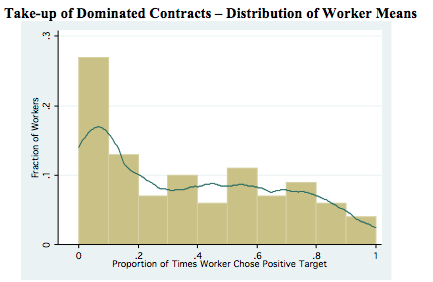
\includegraphics[width=0.8\textwidth]{Figure1_4.png}
\caption{\label{fig:Figure4}}
\end{figure}

If workers were assigned to the control contract that day, they would have missed the target with 9.1 percent of the time.(Table 5,panel A, col.1). In the experiment, workers missed their chosen targets under the option to choose a dominated contract treatment with 2.6 percent of the time (Table 5,panel A, col.1). These results are consistent with the existence of stochastic shocks to output or cost of effort. For instance, anytime there was a probability of network risk or computer issues, all these factors could decrease productivity for rest of the day. This kind of shocks create additional costs for workers beyond the financial penalty, such as having to stay in the office late, in order, to meet the daily targets. Even risk- averse workers work hard to ensure that achieve their target before the shock arrives. All in all, the results in tables 4 and 5 support the view when workers chose their own targets, they did so sensibly-balancing the motivational benefits with the risk of lost earnings- leading them to choose target levels that increased their average earnings.   


\textbf{C. Heterogeneity in Preferences: Correlation between Payday and Contract Effects (Test 3 and 4)}
Author strongly rejects that workers are homogeneous in both effects. The results from payday and contract choices state that at least some of the workers time inconsistent. For instance, 41 percent of workers have 10 percent or larger pay cycle effect. 
In order to test the heterogeneity in payday effects, author regresses production on a payday dummy, worker fixed effects, it is interactions of each worker fixed effect with the payday dummy and standard controls. The \textit{p-value} of the \textit{F-test} coefficient is .000.

Respectively, to test for heterogeneity in treatment effects of contracts, to control used a limited sample and option to choose dominated contract observations and regress production on worker fixed effects, an option to choose a dominated contract assignment dummy, interactions of each worker fixed effect with dummy and standard controls. The \textit{p-value} of the \textit{F-test} of joint significance of the interaction coefficients is .003. 

Preposition 3 predicts that the payday and contract effects will be positively correlated. To test this the effect of payday for each worker is as follows, 
$$Payday effect = \frac{(Mean production  on paydays - Mean production on non paydays)}{Mean production sample}$$. This is a summary that measures a worker's payday effect at the start of the empirical analysis because this measurement does not take a strong ex ante stance on the nature of time inconsistency. On average, workers with an above-average payday effect are 13.8 percentage points more likely to select a positive target and select targets that are 351 fields higher (table 6, panel A).    

High payday effect workers are more likely to show up to work when assigned the option to choose a dominated contract or target imposed. (Table 6, panel B, col.3)
Consequently, it proves that high payday effect workers demand dominated contracts. The estimate of labor supply elasticity is 0.33, the 9 percent intent to treat effect implies that providing high payday effect workers with simply the option to select targets leads to production increases comparable to a 27 percent increase in the piece rate wage. This magnitude corresponds to a 1-year increase in education. Using proposition 2, the treatment on the treated effects allows to bound the level of time inconsistency of the workers that, on the basis of their pay cycle behavior, appear most time inconsistent. When these workers choose dominated contracts, 
\begin{equation}
\frac{\frac{d^I(T)}{d^I(t)}}{\frac{d^I(T-t)}{d^I(0)}}  - 1 \geq  \frac{0.28}{0.33}=.084; 
\end{equation}


It implies that the relative value of the wage benefits to effort costs is 84 percent higher at the time of contract choice than at the time of effort. The workers most affected by paydays, also select more aggressive targets. Author, estimates that high payday effect workers would have missed their selected targets 11.8 percent of the time had they been under the control contract and actually miss them 5.2 percent of time. Consistent with proposition 4, when high pay day effect workers are closer to their payday, and self - control problem is therefore smaller, the treatment effect of the option to choose a dominated contract is smaller. In contrast, low payday effect workers, who are not affected by the dominated contract treatments, exhibit no detectable trends over the pay cycle. 

\textbf{D. Learning over Time} 
As workers gain experience, do they learn about the value of dominated contracts or perhaps find other ways around their self-control problems? 
\begin{figure}[h]
\centering
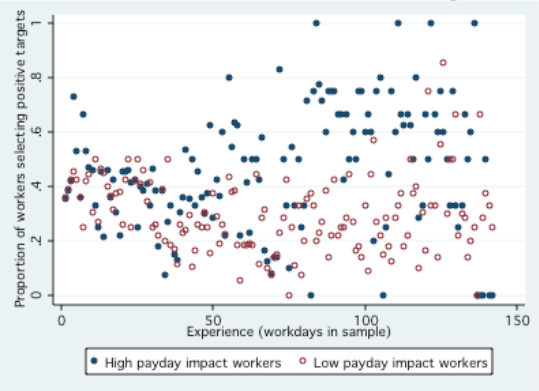
\includegraphics[width=0.8\textwidth]{Figure1_5.png}
\caption{\label{fig:Figure1.5}}
\end{figure}

In this figure below, it shows an experience (number of workdays in the experiment) against proportion of workers choosing positive targets(dominated contracts), where high pay day effect workers are shown in closed circles and low payday effect workers are shown in open. From the figure, mean take-up rates of dominated contracts among the two groups are initially similar. As workers gain experience there exist divergence, in other words, low payday effect workers decrease take-up of dominated contracts while high payday effect workers increase take-up. After 60 days of experience, high payday effect workers are 20.6 percentage points, or 73 percent, more likely to select positive targets than low payday effect workers, \textit{p-value is .000}.  

As a result, the impact of paydays on output does not change with experience, suggesting that underlying self-control problems do not change over time. But, the treatment effect of giving workers option to choose dominated contract grows with experience. 

\textbf{Morning and Evening choice (Test 5)}
In the contrary to initial expectations, on average across the sample, workers didn't select higher targets in the evening before the work than in the morning of work. Analysis suggest that in the evening before  the workday, workers faced two types of uncertainty that were partially resolved by the morning of the workday. First, the network fluctuations affected the rate at which workers could send data entered from an image to the central server and retrieve the next image for entry. Waiting time is ranged from 1 second to over 5 minutes. Such network shocks greatly affected productivity for these computers. Assignment to the more uncertain computers decreases mean output by 313 fields or 6 percent, a magnitude that corresponds to an 18 percent reduction in the piece rate based on your elasticity estimate. 

When workers are assigned to a computer that is not as sensitive to network fluctuations, they are 6.6 percentage points more likely to choose a dominated contract when given the choice the evening before production than the morning production. However if they were assigned to bad computer, they are 1.6 percentage points less likely to choose a positive target in the evening than the morning.  

Second type of uncertainty is that many workers faced issue with commute and arrival time, which was resolved by the time they arrived to work in the morning. 

When uncertainty is lower and similar between the evening before and the morning of work, workers are more likely to choose dominated contract in the evening. However, if uncertainty is high the evening before the production but is reduced by the next morning, take-up is higher in the morning. Here the results shows that contract demand can interact with uncertainty. 

\subsection{Critical Assessment}
The central criticism of the model - authors aimed to find out whether the results are consistent with a self-control agency model. But there are still remained questions to be investigated such as: could they be explained within the context of standard exponential discounting model? Authors argue that while other models could explain any one result, self-control problems are required to fit the full pattern results: the production increases on paydays, sustained demand for dominated contracts, treatment effects of contract choice, the correlation between the payday effects and demand for dominated contracts.  
First, could workers chose dominated contracts because they are confused? The answer is no, because during the training period, workers were assigned to various contracts and also tested their comprehension using contract quiz, where the mean score was 93 percent. Take-up is not being driven by those who have worse understanding of contracts: quiz performance is positively correlated with take-up and education strongly predicts take-up. Second, could workers choose dominated contracts to signal ability to employers? Since the employer observes production directly, there is no reason to believe that a worker who is productive under the control contract is not more impressive than one who needs to rely on a dominated contract. In addition, it is unclear why workers with larger payday effects should be more likely to signal ability, or why workers more likely to signal ability the evening before the workday than the morning when assigned to good computers. 
Could weekly income targeting explain the payday effects? Income targeting implies a sharp decrease in marginal utility for income levels above the target. 
Depending on the end-line survey, many workers expressed a desire for rules to help them work harder under pure piece rate: 78 percent of workers agreed that on some days they don't work as hard as they would like to and 87 percent agreed with that they wish to have better attendance at work. Some workers expressed demand for workplace rules to increase effort. For instance, 70 percent agreed with if there were rules against being absent because it would help them come to work more often. Therefore, I believe that the workplace policy should be more strict as it will lead to the increase in production.  If workers come to work late  or don't attend then the punishments have to be  strict and clear, which sometimes may lead to employees getting fired. 



\section{Paper 2 "Alcohol and Self - Control: A field experiment in India"}
\subsection{Summary}
Heavy alcohol consumption reduce wealth accumulation and leads to poverty by affecting savings decisions, insurance take - up, human capital investments and earnings. Therefore, I asked myself whether such effects are present and economically meaningful in practice? Are individuals aware of the cost of alcohol consumption?

Second paper tests the impact of alcohol on savings behavior. To figure out the relationship between them, an experiment was conducted, where 229 individuals participated with low income, high return savings opportunity and randomized incentives for sobriety. The incentives to remain sober increased individuals sobriety  and decreased consuming alcohol during their daytime study office visits. However, overall alcohol consumption and expenditures remained unchanged. Because individuals just shifted their drinking to later times of the day. In addition, the daily earnings from work were significantly small, therefore, offering incentives for sobriety increased individuals savings by about 60 percent compared to control group, who received similar average study payments independent of their alcohol consumption. The relationship between the effects of sobriety incentives and commitment savings is that they are substitutes in terms of effect on savings.    
Moreover, this paper contributes to the literature on poverty and self - control,\cite{Fisher30}. This research lines have largely sought to explain choices between overall levels of current and future consumption, rather than to understand how and whether specific goods may cause time - inconsistent preferences. In contrast, this paper argues that focusing on vivid temptation goods may not be the only effective way to solve how individuals overcome their self - control problems regarding the consumption of goods but, in the case of alcohol, may also reduce self - control problems in other domains. 


As a result, this paper tells that alcohol itself can make worse bias now and later create further self-control problems on other fields.  It is common of high level of alcohol consumption among poor families and individuals. Consequently, alcohol consumption has economic effects on the income, because it harms mental processes and decision making in the future. Flowingly, we will see the a three - week experiment that alcohol impacts on savings and self - control. 


The results from experiment showed that increased sobriety is associated with the absolute increases in participants savings during their study office visits. However, it remained to be investigated whether modified commitment contracts are able to help individuals reduce their overall drinking if they desire so. The key point of such contracts might be a better and more continuous monitoring by themselves using technologies.  



\subsection{Experimental Design}

\textbf{Overview of Experimental Design}:
The experiment was conducted between April and September 2014. 229 cycle-rickshaw peddlers took a part and were asked to visit study office every day for three weeks each. All along, participants completed a Breathalyzer test and a short survey on labor supply, earnings, and expenditure patterns on the previous day, and alcohol consumption both on the previous day and on the same day before coming to the study office. To measure the impact of increased sobriety due to financial incentives on savings behavior, participants had all opportunity to save money at the study office. Moreover, they were assigned to different treatment groups, where some of them were offered a financial incentives to visit the office sober and remaining part of participants were paid for coming to the office regardless of their alcohol consumption. Next is to observe the interaction between sobriety incentives and commitment savings, participants were allowed to withdraw their savings only at the end of study. Last but not least, to identify the alcohol, self - control participants had a choice between incentives for sobriety and unconditional payments.  

\textbf{Recruitment and Screening}
The main goal of screening was \textit{a. It has to be homogeneous sample }, \textit{b. be able to for efficient communication} and \textit{c. limit unrelated errors }. Participants could only proceed if they meet screening criteria such as : \textit{1. Males between 25 and 60 years old, inclusive}, \textit{2. Fluency in Tamil, the local language}, \textit{3. had worked at least five days per week as a rickshaw puller during the previous month}, \textit{4. had lived in Chennai for at least six months}, \textit{5. self reported daily average hard liquor daily consumption of 0.7 to 2.0}. 

\textbf{Selection}
From the observational survey, the majority of individuals were able and willing to proceed next stage. \textit{Table C.1}. 64 percent of individuals were eligible and decided to visit the study office to complete the survey.


\textbf{Timeline and Treatment Groups}
In figure 2 indicated the whole period of study, the different activities and treatment conditions. During the screening process, Phase 1, all participants were paid at constant rate Rs.90 (1.50 US dollars) regardless of their alcohol content(BAC). After 4 days they were randomly distributed to the following groups : \textit{ 1) Control Group}. In this group, participants continued with payment schedule from Phase 1. \textit{2) Incentive Group}. They were paid for visiting the office Rs.60 (1 US dollar) and additional Rs.60 if they are sober and \textit{3) Choice Group}. In this group, they were given same incentives as in second group, then on day 7 and day 13 were offered for subsequent week, to know whether they preferred to continue receiving the same incentives or to receive unconditional payments ranging from Rs. 90 to Rs.150. 

\begin{figure}[h]
\centering
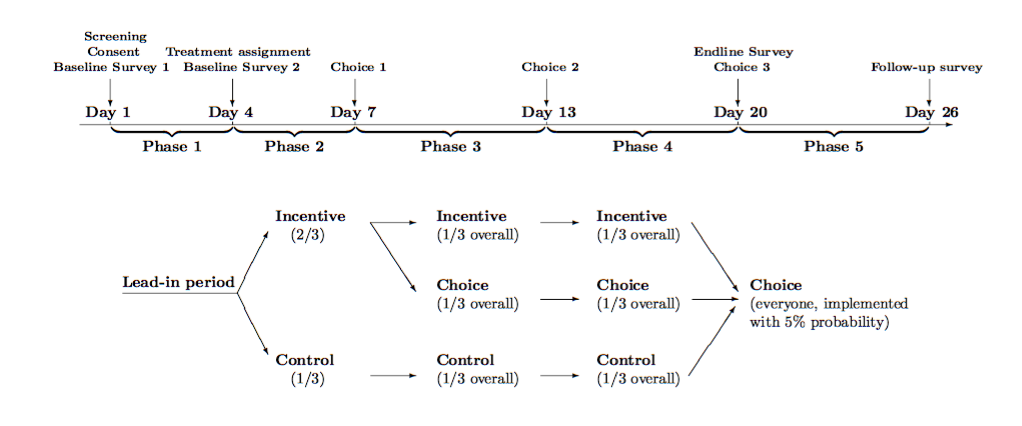
\includegraphics[width=1\textwidth]{FIG_Experimental_Design.png}
\caption{\label{fig:Figure2}}
\end{figure}

\textbf{Outcomes of Interest, Savings Treatments, and Lottery}
Three main outcomes of interest described in this study: \textit{1) Alcohol consumption and expenditures}, where was collected daily data during the study office by measuring participants Blood alcohol content(BAC); \textit{2) Savings Behavior}, where participants could choose either matching contribution(savings bonus) rate or commitment savings; and \textit{Lottery}, if participant arrived at the study office on a assigned day, he could win a voucher for Rs.30 or Rs.60 with a small probability each.

\subsection{Does Alcohol Consumption Affect Savings Decisions?}
This section discusses about the evidence that intense alcohol intoxication distorts choice and thereby causes self - control problems in savings decisions. Here, author argues that increasing sobriety impacts savings behavior beyond effects on income net of alcohol expenditures. In figure C.3, we can see strong correlation between daily amounts saved at the study office and blood alcohol content (BAC) measured during the same office visits, which holds both across Control Group participants and with in same individuals overtime. 

\begin{figure}[h]
\centering
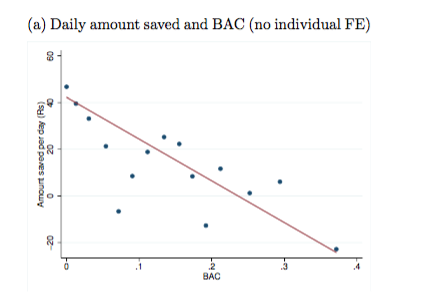
\includegraphics[width=0.7\textwidth]{FigureC3.png}
\caption{\label{fig:FigureC3}}
\end{figure}


\textbf{The Impact of Financial Incentives on Alcohol Consumption}
Table 1 shows that financial incentives significantly reduced daytime drinking but they had only a moderate effect on overall drinking. Moreover, Financial incentives increased sobriety during the day, as measured by the fraction of individuals who visited the study office and had zero Breathalyzer test result among all participants in the respective treatment groups. (Upper panel of Figure 3). The columns 7 through 12 on same table shows us that the estimated treatment effect on overall drinking is lower than the estimated effect on daytime drinking. First of all, both treatments reduced reported overall alcohol consumption by about 0.3 standard drinks per day. Next is the reduction on extensive margin of drinking was small at best (columns 9 and 10 ). Lastly, the treatment effect on reported overall alcohol expenditures is about Rs. 5 to 10 per day (columns 11 to 12), with point estimate of Rs. 9.8 for the pooled treatment effect. From the observation, we see that these results provide evidence that subjects who responded to the incentives mostly shifted their alcohol consumption to later times of the day rather than reducing their overall consumption or not drinking at all. The impact on the incentives reduced drinking before study office visits but the impact on overall drinking was small. These results show us that the incentives shifted in the distribution of the timing of individuals. Approximately, 10 percent of participants in the Incentive Group and Choice Groups just delayed their drinking time. 
\begin{figure}[h]
\centering
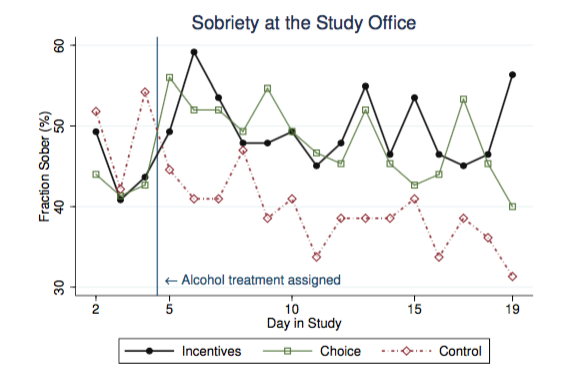
\includegraphics[width=0.8\textwidth]{Figure3.png}
\caption{\label{fig:Figure3}}
\end{figure}

\textbf{The Role of Differential Attendance}
Across the treatment groups, the attendance was indifferent. It didn't cause the estimated effect of incentives on sobriety. Overall, attendance was 88.4 percent and 85.4 percent in post treatment assignment. 

\subsection{Did Increased Sobriety Change Savings Behavior?}
When the incentivized period started, individuals in Incentive Group saved 46 percent (Rs.446) and Choice Group saved 65 percent(Rs.505) more than Control Group(Rs.306). Figure 5 shows us how average amounts saved were nearly identical across treatment groups.

\begin{figure}[h]
\centering
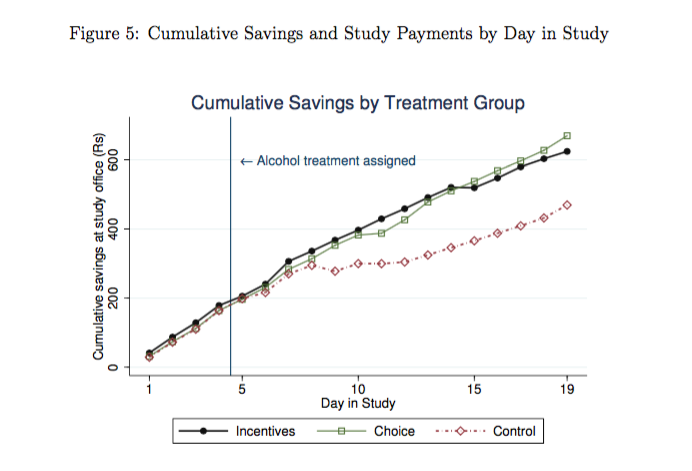
\includegraphics[width=1\textwidth]{Figure5.png}
\caption{\label{fig:Figure5}}
\end{figure}

\textbf{The effect of changes in Income Net of Alcohol Expenditures}

In this paragraph, author discussed whether sobriety incentives impact reflect changes in individuals savings decisions for a specific given recourses. Making a lottery is one of the ways to estimate \textit{the Marginal Propensity to Save(MPS)}. Table C.7 shows the regressions of daily amounts saved on a dummy for the pooled alcohol treatment as well as the amount won in the lottery on the previous day, and interactions of the treatment dummies with the lottery amount. These regressions show a marginal propensity to save of 0.15 to 0.19 in the Control Group, and 0.28 to 0.40 in the pooled alcohol treatment groups. 
Now, let's see the effect of \textit{Reduced Alcohol Expenditures on Savings}. It says that even small reductions in alcohol consumption can significantly increase their overall income. Using the implied expenditure reduction based on reported physical quantities consumed, treatments decreased alcohol expenditures by between Rs.4.7 to Rs.10.7 per day. If these estimates combined with the estimated marginal propensity to save available resources of 0.19 in the Control Group(column 6 same table)
It implies that reduced alcohol expenditures accounted for Rs.089 to Rs.2.03 of the increase in savings. The combination of the effect estimations gives the assessment of increase in savings explained by mechanical effects. If subtract \textit{the contribution of reduced alcohol expenditures(Rs.2.03)} and \textit{the contribution of increased earnings(Rs.2.05)} from the starting point of overall treatment effect, it gives us unexplained treatment effect of Rs.6.95. These calculations tell that increased sobriety indeed impacted savings behavior for given resources. 
 
 \textbf{Household Resources and Complementary Consumption}
In this subsection described two additional concerns: First is the increase in savings at the study office due to increased sobriety may have to come at the cost of reduced household resources. Table C.8 shows that sobriety incentives increased money given to wives by about Rs.17.5. Second, reduced alcohol consumption during the day or overall may have lowered expenses on complementary consumption goods such as tobacco.  

\subsection{Are Sobriety and Commitment Savings Substitutes?}
This section presents a simple model of a present-biased consumer as in \cite{Laibson97} to formalize this intuition. Then author considers two specific features of the model. First, the impact of commitment savings is an inverse U-shaped function in present bias for sophisticated individuals. The impact of commitment savings devices is lowest for individuals without present bias (beta =1) and for the most present-biased individuals (beta =0). Second, for empirically relevant parameter range of beta> 0.5, an increase in beta lowers the impact of commitment savings on savings. 


\textbf{A Simple Model}
A consumer lives for three periods. In Period 1 he receives an endowment $Y_1$. There are no other incomes sources in Periods 2 and 3, but the consumer is paid a matching contribution of \textit{M} times the amount saved by the start of period 3. In periods \textit{t} = 1,2, he has to decide how to allocate his available resources into instantaneous consumption $c_t$ or savings. The instantaneous utility function $u(c_t)$ is increasing and concave: $u\prime(.)$ >0 and $u\prime\prime(.)$<0. In period 1, individual maximizes $U_1(c_1,c_2,c_3) \equiv u(c_1) + \beta [u(c_2)+u(c_3)]$ and in Period 2 he maximizes $U_2(c_2,c_3) \equiv u(c_2) + \beta u(c_3)$. 

Consider first a model \textit{without commitment savings}. In Period 3, the individual will consume the entire amount saved plus the matching contribution: $c_3=(Y_1-c_1-c_2)(1+M).$ In Period 2, the individual takes $c_1$ and maximizes 
$$\max_{c_2} u(c_2)+\beta u((Y_1-c_1-c_2)(1+M)) $$
First Order Condition(FOC): $u\prime (c_2)\beta(1+M)u\prime((Y_1-c_1-c_2)(1+M)).$

Now, consider second model is \textit{commitment savings,} where any money is saved in Period 1 can not be withdrawn until Period 3. The Period 1 self would like to set $u\prime(c_2)=(1+M)u\prime(c_3)$. However, in the absence of commitment savings, the period 2 self deviates from this, i.e chooses $c_2$ such that $u\prime(c_2)=\beta(1+M)u\prime(c_3)$, hence, consumes more than the Period 1 self would like. Therefore, this creates demand for commitment for Period 1 self. 

The individual will consume $c_1$ and deposit $c_3$ into the commitment savings account such that $u\prime(c_1)=\beta u\prime(c_2)=\beta(1+M)u\prime(c_3)$ subject to budget constraint. Hence, the solution is described by the following equations: $$u\prime(c_1)=\beta u\prime(c_2)$$ $$u\prime(c_2)=(1+M)u\prime(c_3)$$

These two solutions clarifies the relationship between present bias and commitment savings. Since the commitment savings device makes both the Period 1 and 2 selves consume a smaller share of their available resources $Y_1$ and $Y_2$, commitment option increases savings iff $0<\beta<1$. Commitment savings has no impact at $\beta=1$ and $\beta ->0$. 



\subsection{Do Individuals want to reduce their Drinking?}
In this discussion part author considers the extent to which self-control problems contributed to individuals demand for receiving incentives for sobriety. Individuals in Choice Group, after receiving incentives for three days, were asked to choose between incentives to arrive sober and different amounts of unconditional payments. \textit{Dividing choice points into several phases.} This structure allows to investigate whether individuals in the Choice Group changed their choices over time and whether receiving incentives in earlier phases of the study affected individuals demand for commitment. The high demand for commitment might be explained by several of factors. First, many individuals in the sample had been drinking alcohol for many years and their beliefs regarding their future drinking were fairly sophisticated. Next, many individuals expressed a strong desire to reduce their drinking surveys. Third, individuals had been given an experience with the incentives before making their choices. Fourth, commitment contracts were implicitly defined via choices of different structures of study payments rather than asking individuals explicitly whether they were willing to give up money that they earned. Consequently, individuals may have perceived their choices as decisions between various gains rather than considering potential losses in study payments due to commitment choices. 

\subsection{Critical Assessment}
In the article, "Alcohol Self - Control", author Frank Schilbach, discusses sobriety incentives on alcohol consumption. Author makes strong statement that the incentives significantly reduce daytime drinking, which in turn increases savings by 60 percent. Moreover, over half of the study participants were willing to sacrifice money to receive incentives to remain sober. He also gave an excellent evidence to support the claim that economic implications of the cross - randomization of sobriety incentives and commitment savings may have a greater impact in the immediate future.  

The author claims that the results show the increasing sobriety reduced self control. In other words, alcohol is a key temptation good for this population.  Reducing alcohol consumption diminishes the need for commitment savings. However, the intervention reduced only the overall alcohol consumption and expenditures. The next argument that the author suggests is that there was an upper bound of how much individuals were able to or wanted to save. However, average daily savings were below the savings limit of Rs.200 per day. Moreover, all individuals received relatively large study payments in addition to their earnings outside of the study, which appear to have been largely unaffected by the study. Accordingly, the majority of individuals would have been able to increase their savings if they had preferred to do so. However, increasing the matching contribution rate didn't influence the complement to increased sobriety. 

\begin{figure}[h]
\centering
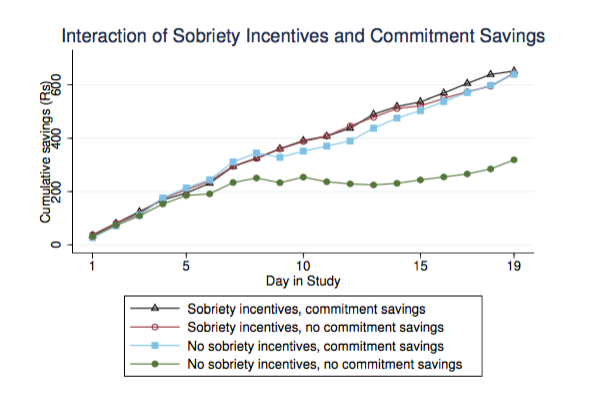
\includegraphics[width=0.9\textwidth]{Figure6.png}
\caption{\label{fig:Figure6}}
\end{figure}


The immediate and long -term economic impacts toward improved policymaking will be to collect higher - quality and more systematic data on alcohol consumption patterns in developing countries. It should include more frequent measurements and data on intoxication levels. Later, these data results will help to assess the consequences of different policies intended to reduce drinking as well as to see the impact of alcohol consumption on labor market outcomes, decision - making, family outcomes and poverty. First, and attractive option is to "sin taxes", is an excise tax on socially harmful goods, to prevent self - control problems. \cite{Gruber01}. If poor individuals are more price - elastic or more present - biased compared to rich individuals, than ""sin taxes" can be more progressive. The results from the study shows that regressiveness of taxing alcohol maybe reduced by effects of reduced drinking on earnings and savings.  
Second option is a more extreme policy - prohibition. Since the distribution of alcohol consumption is heavily skewed, prohibition may be particularly attractive policy option, with the majority of the population abstaining from alcohol and relatively large share among the drinkers consuming alcohol excessively. In contrast, prohibition may result in other unintended consequences such as crime and corruption\cite{Thornton91}.


\subsection{Ideas for future work}
There are still remained questions to be investigated whether modified commitment contracts are able to help individuals reduce their overall drinking if they so desire.  





\newpage
\bibliographystyle{alpha}
\bibliography{sample}

\newpage
\section{Statutory Declaration}
I declare that I have authored this thesis independently, that I have not used other than the declared sources / resources, and that I have explicitly marked all material which has been quoted either literally or by content from the used sources.

\newpage
\section{Appendix}

\begin{table}[h]
\centering
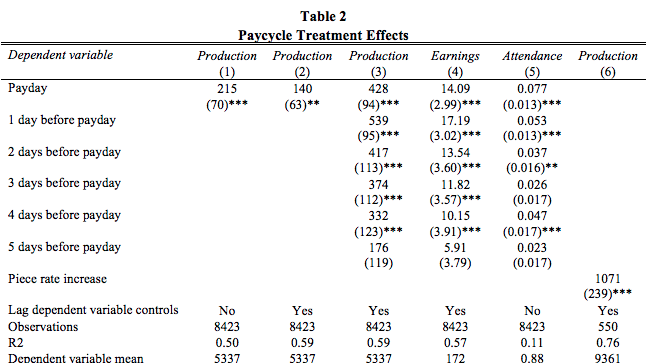
\includegraphics[width=0.8\textwidth]{Table2.png}
\caption{\label{fig:Table2}}
\end{table}

\begin{table}[h]
\centering
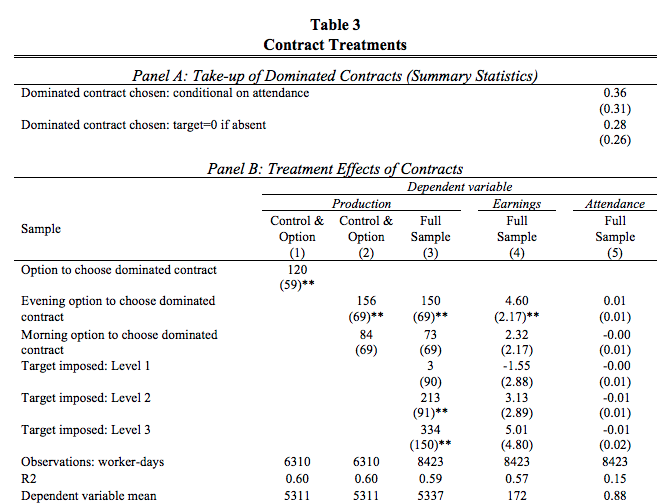
\includegraphics[width=0.7\textwidth]{Table3.png}
\caption{\label{fig:Table3}}
\end{table}

\begin{table}[h]
\centering
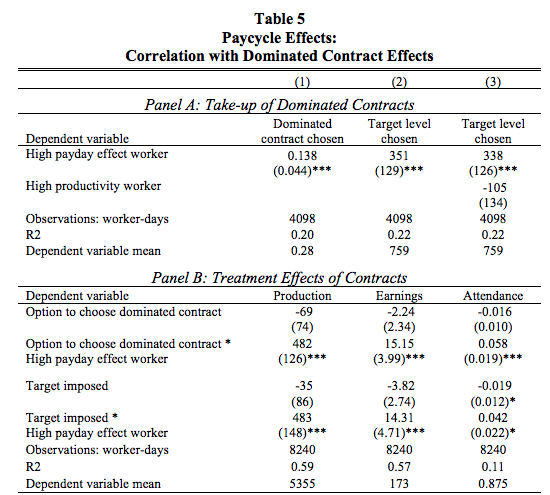
\includegraphics[width=0.7\textwidth]{Table5.png}
\caption{\label{fig:Table5}}
\end{table}
\begin{table}[h]
\centering
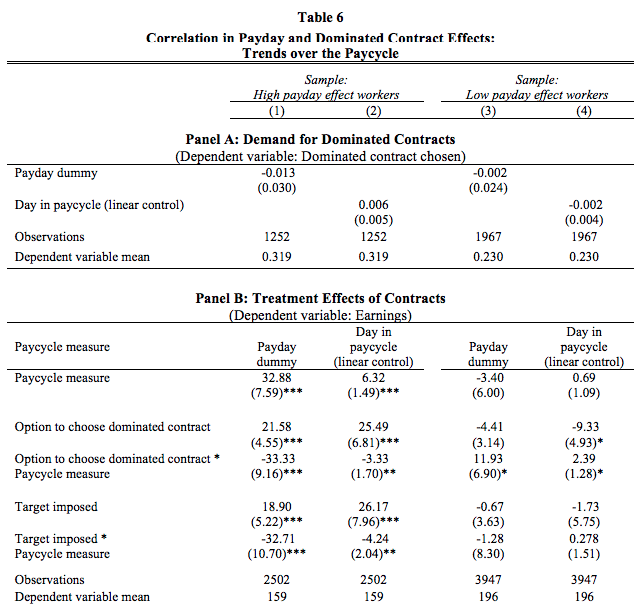
\includegraphics[width=0.7\textwidth]{Table6.png}
\caption{\label{fig:Table6}}
\end{table}
\newpage
\end{document}
\end{document}